%
% main.tex -- Paper zum Thema deconvolve
%
% (c) 2019 Hochschule Rapperswil
%
\chapter{Wavelet-Deconvolution\label{chapter:deconvolve}}
\lhead{Wavelet-Deconvolution}
\begin{refsection}
\chapterauthor{Manuel Tischhauser}

\section{Einleitung}
\rhead{Einleitung}
%
% einleitung.tex
%
% (c) 2018 Prof Dr Andreas Müller
%
\chapter*{Einleitung\label{chapter:einleitung}}
\lhead{Einleitung}
\addcontentsline{toc}{chapter}{Einleitung}
Zeitabhängige Signale können verstanden werden als Funktionen $t\mapsto f(t)$
mit $t\in\mathbb R$.
Die Analysis lehrt eine Reihe von Methoden, wie man mit solchen
Funktionen arbeiten kann.
Dies ist jedoch eine mathematische Idealisierung.
In der Praxis kennt man nur das Resultat eines Abtastprozesses, wo
der Funktionswert $f(t_k)$ für diskrete Werte $t_i=t_0 + k\Delta t$
ermittelt wird.
Insbesondere gehen alle Informationen über den Verlauf einer Funktion $f(t)$
zwischen den Abtastpunkten $t_k$ verloren.
Trotzdem führt daran nichts vorbei, denn nur auf diese Art ist es möglich,
Signale in einem digitalen System zu verarbeiten.

Die Methoden der Analysis sind für folgen von Abtastwerten $x_k=f(t_k)$
fast nutzlos.
Sogar das Konzept der Frequenz ist fragwürdig, denn ein Sinus-Signal
$s(t)=\sin(2\pi t/\Delta t)$ nimmt auf allen Abtastpunkten $t_k$
den Wert $s(t_k)=\sin(2\pi t_0/\Delta t+2\pi k)=\sin(2\pi t_0/\Delta t)$
den gleichen Wert an.
Allgemeiner: ein Signal mit der gleichen Frequenz wie die Abtastfrequenz
ist nicht von einem konstanten Signal unterscheidbar.
Die Signalverarbeitung verlang daher nach einem Satz von Werkzeugen, die
einerseits mit dieser Schwierigkeit fertig werden, aber andererseits auch
in der Lage sind gut verstandene technische Prozesse wie das Ausfiltern
bestimmter Frequenzbereiche adäquat zu beschreiben.

Das übliche und für den Ingenieur naheliegende Werkzeug ist die 
Fourier-Theorie, die ursprünglich als analytisches Hilfsmittel zur Lösung
von Differentialgleichungen entwickelt wurde.
Sie machte erstmals möglich, ein Signal über die darin vertretenen
Frequenzen zu charakterisieren und zu manipulieren.
Mit der Entwickung der schnellen Fourier-Transformation
(Fast Fourier Transform, FFT) wurde ihr praktischer Einsatz in digitalen
Problemlösungen möglich.
Sie bringt die neue Idee in die Diskussion, ein Signal als Überlagerung
von Beispielfunktionen zu betrachten, die besonderes einfach zu
verstehen sind.
Konkret sind dies die Funktionen $\sin kt$ und $\cos kt$ mit
$k\in\mathbb N$ bei der Analyse periodischer Signale,
oder allgemeiner die Funktion $t\mapsto e^{ikt}$ mit $k\in\mathbb Z$
bei beliebigen Signalen.
Die daraus entwickelte Theorie ist zwar sehr reichhaltig und auch erfolgreich,
aber doch in einem Punkt unbefriedigend.
Die Fourier-Transformation liefert zu einem Signal detaillierte Information
über die darin enthaltenen Frequenzen, dafür gehen aber Informationen
darüber verloren, wann interessante Ereignisse eingetroffen sind.
Die Information ist nicht ganz verloren, da sie immer noch in den Phasen
der Koeffizienten stecken, aber sie sind für alle praktischen Zwecke 
nicht mehr nutzbar, da nur über eine Rücktransformation wieder erschliessbar.

Es stellt sich daher die Frage, ob es Möglichkeiten der Analyse von Signalen
gibt, die nicht so radikal sind.
Enthält ein Signal hohe Frequenzen, dann ändert sich das Signal rasch.
Ein kurzes Ereignis passt auf diese Beschreibung, aber eine wesentliche
Eigenschaft ist damit nicht beschrieben, nämlich wann es statt gefunden hat.
Kann man Informationen über die in einem Signal vertretenen Frequenzen gewinnen,
ohne auf Information darüber verzichten zu müssen, wann diese Ereignisse
eingetreten sind?

Für eine umfassende Antwort müssen mehrere Teilfragen untersucht werden.
\begin{enumerate}
\item
Welche Arten von Vergleichssignalen soll man verwenden, um solche kurzlebigen
Ereignisse zu beschreiben?
Die trigonometrischen Funktionen sind zweifellos naheliegend und ihre
analytischen Eigenchaften einladend, doch ihre unendliche Ausdehnung entlang
der Zeitachse torpedieren von vornherein die Möglichkeit der zeitlichen
Lokalisierung von interessanten Ereignissen.
Gibt es Funktionen, die ähnliche oszillatorische Form haben
aber trotzdem über hilfreiche analytische Eigenschaften haben?
\item
Wie vergleicht man ein gegebenes Signal mit einem Vergleichssignal?
In der Fourier-Theorie lernt man einen ausgedehnten Satz von Integralformeln
zur Berechnung der Fourier-Koeffizien\-ten.
Wie müssen diese verallgemeinert werden?
\item
Wie rekonstruiert man das Signal aus dem Resultat der Analyse?
In der Fourier-Theorie lernt man Summenformeln für die Fourierreihen
und Integralformeln für ausgedehnte Signale, doch wie ist das für 
die neuen Vergleichsfunktionen umzusetzen?
\item
Die Praxis arbeitet mit diskreten Signalen. 
Wie lässt sich die Analyse diskretisieren?
Unter welchen Voraussetzungen ist die Rekonstruktion des Signals
aus der diskreten Analyse möglich?
\item
Das Verfahren ist nur dann praktisch einsetzbar, wenn sowohl die Analyse als
auch die Synthese mit effizienten numerischen Algorithmen möglich sind.
Diese Algorithmen müssen ausserdem stabil sein, d.~h.~kleine Störungen in
den Input-Daten oder Rundungsfehler während der Durchführung des Verfahrens
dürfen sich nicht zu unbrauchbaren Resultaten aufschaukeln.
\item
Welche Vergleichssignale sind für welchen Anwendungszweck geeignet?
\end{enumerate}
Die nachkommenden Kapitel versuchen, Antworten auf diese Fragen zu
geben.

In Kapitel~\ref{chapter:geometrie} wird gezeigt, wie der Vergleich
von Funktionen gleichbedeutend ist mit dem Skalarprodukt von Vektoren.
Daraus entwickelt sich dann die Theorie der Hilberträume, der
unendlichdimensionalen komplexen Vektorräume mit Skalarprodukt.
% Diese bilden den geometrischen Rahmen, in dem man die ganze 

Die bekannte Fourier-Theorie wird im Kapitel~\ref{chapter:fourier} in
den neuen Rahmen des Hilbertraumes eingeordnet.
Es demonstriert, wie die Hilbertraumtheorie die Vielfalt der vielen
verschiedenen Varianten der Fouriertheorie vereinheitlicht.

Das Haar-Wavelet ist das älteste bekannte Wavelet.
Es ist einfach und übersichtlich und kann als Beispiel für die
Phänomene dienen, die bei komplizierteren Wavelets nicht so leicht
zu verstehen sind.
Es wird in Kapitel~\ref{chapter:haar-wavelet} im Detail besprochen.

Die stetige Wavelet-Transformation analysiert ein Signal auf höchst
redundante Art.
Die Hilbert\-raum\-theorie wird in diesem Kapitel~\ref{chapter:cwt} hier
erstmals allgemeiner angewendet.
Wir lernen die Be\-ding\-ungen kennen, die nötig sind, damit ein Signal
aus seiner Wavelet-Transformation rekonstruierbar ist.
Wir geben sogar eine Formel für die Rekonstruktion an.

Bei der Diskretisierung geht Information verloren.
Das in Kapitel~\ref{chapter:shannon} diskutierte Abtast-Theorem
von Shannon gibt an, unter welchen Voraussetzungen das Signal trotz
des Informationsverlustes rekonstruierbar bleibt.

Die diskrete Wavelet-Transformation überträgt die stetige
Wavelet-Transformation auf abgetastete Signale.
Der Begriff der Multiskalen-Analyse wird in Kapitel~\ref{chapter:msa}
dazu verwendet, die angemessene Diskretisierung im ``Frequenzraum''
zu finden.

Aus der Multiskalen-Analyse lassen sich auch die schnellen Algorithmen
ableiten, welche Wavelets überhaupt erst praktisch nützlich machen.
Diese Algorithmen werden in Kapitel~\ref{chapter:algo} hergeleitet.

Selbst mit einer Multiskalen-Analyse brauchen die Algorithmen noch nicht
perfekt zu sein.
Schon bei der Fourier-Transformation war das Problem, dass zur Berechnung
der Fourier-Trans\-for\-ma\-tion alle Input-Daten notwendig sind.
Dies bedeutet, dass das Transformationsresultat erst verfügbar ist,
wenn das ganze Signal abgetastet ist.
Damit sind Verarbeitungen in Echtzeit von vornherein ausgeschlossen.
Ein Ausweg besteht darin, dass die Transformationsoperationen sich auf
einer nur sehr kleinen Anzahl Samples ausführen lassen.
Genau dies wird erreicht, wenn die verwendeten Wavelets einen kompakten Träger
haben.
Solche Wavelets wurden von Ingrid Daubechies in den neunzehnachtizger
Jahren konstruiert und waren massgebend für den schnellen Siegeszug 
der Wavelet-Transformation in den Anwendungen.

Natürlich sind die Daubechies-Wavelets nicht die einzigen praktisch
nützlichen Wavelets.
Die verbleibenden Kapitel zeigen eine Reihe von alternativen Wavelets,
zum Beispiel in Kapitel~\ref{chapter:spline} die Spline-Wavelets.
Das Haar-Wavelet ist sowohl das einfachste Daubechies-Wavelet als auch
das primäre Spline-Wavelet.











\section{Eindimensionales Signal}
\rhead{Eindimensionales Signal}
Betrachtet werden die beiden Funktionen, welche in Abbildung \ref{deconvolve:1d} dargestellt sind.
\begin{figure}
\centering
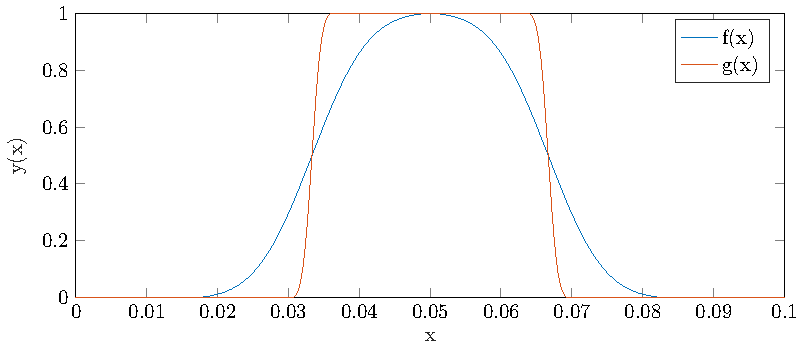
\includegraphics[width=0.9\textwidth]{./papers/deconvolve/pictures/1d.pdf}
\caption{Funktionen für die eindimensionalen Versuche\label{deconvolve:1d}}
\end{figure}
Eine stetige Wavelet-Transformation von $f(x)$ mit dem Haar-Wavelet ist in \ref{deconvolve:y1_cwt} abgebildet.
Lässt man nur bestimmte Dilatationen ($a=2^n, n\in \mathbb{N}$) bzw. die orangen \glqq Zeilen\grqq{} der stetigen Transformation zu, werden die Level der diskreten Transformation sichtbar.
Jedes Level tiefer wird das Wavelet \glqq halbiert\grqq{} und somit die Auflösung höher.

\begin{figure}
\centering
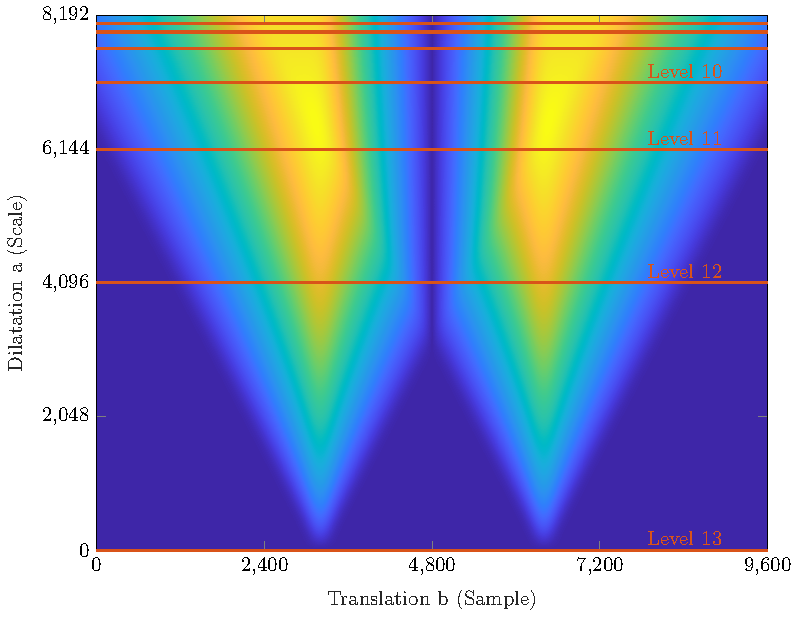
\includegraphics[width=0.9\textwidth]{./papers/deconvolve/pictures/y1_cwt.pdf}
\caption{CWT von $f(x)$ (Abbildung \ref{deconvolve:1d})\label{deconvolve:y1_cwt}}
\end{figure}

In \ref{deconvolve:y1_cwt} sind der Übersicht halber nur die Level 7--13 eingezeichnet. 
Die Abbildung der stetigen Transformation dient hier nur zur Visualisierung, für die eigentliche Umsetzung wird nur noch mit der diskreten Transformation auf den Level 1-13 gearbeitet.

Zu beachten ist, dass die Beschriftung der $y$-Achse (Scale) nicht direkt der Dilatation $a$ entspricht.
Je tiefer der Wert, desto mehr ist das Wavelet gestaucht oder anders gesagt, tiefe Frequenzen befinden sich oben, hohe unten.

Die Funktion $f(x)$ aus \ref{deconvolve:1d} wird mit dem Haar-Wavelet $\psi_{a,n}(x)$ analysiert.
Mit $a$ wird dabei natürlich die Dilatation und mit $n$ die diskrete (sampleweise) Translation bezeichnet.
Für jede Verschiebung $n$ erhalten wir einen Koeffizienten $cf_{k,n}$, wobei der Index $k\in[1,2,...,13]$ für das jeweilige Level steht. 

Mathematisch ausgedrückt beutetet das
\begin{align*}
	cf_{13,n} =& \frac{1}{\sqrt{2^0}}\int_{-\infty}^{\infty}f(x)\cdot\psi_{2^0, n}(x)\,dx = \int_{-\infty}^{\infty}f(x)\cdot\psi_{1, n}(x)\,dx\\
	cf_{12,n} =& \frac{1}{\sqrt{2^1}}\int_{-\infty}^{\infty}f(x)\cdot\psi_{2^1, n}(x)\,dx = \frac{1}{\sqrt{2}}\int_{-\infty}^{\infty}f(x)\cdot\psi_{2, n}(x)\,dx\\
	\vdots\\
	cf_{1,n} =& \frac{1}{\sqrt{2^{12}}}\int_{-\infty}^{\infty}f(x)\cdot\psi_{2^{12}, n}(x)\,dx = \frac{1}{64}\int_{-\infty}^{\infty}f(x)\cdot\psi_{4096, n}(x)\,dx.
\end{align*}

Nun kann aus all den erhaltenen Koeffizienten $cf_{k,n}$ ein Vektor $cf_k$ gebildet werden
$$cf_k = \left(\begin{array}{c}
	cf_{k,0}\\
	cf_{k,1}\\
	\vdots\\
	cf_{k,n}\\
\end{array}\right),$$
mit welchem dann so kompakt weiter gearbeitet wird.
Der Vektor aus der Koeffizienten $cg_{k,n}$ von $g(x)$ wird analog dazu $cg_k$ genannt.

Zu erwähnen ist noch, dass $n$ von der Länge der analysierten Funktion und vom jeweiligen Level abhängig ist.
Ist $f(x)$ wie in diesem Beispiel 9600 Samples lang, besteht $cf_1$ aus 4800 und $cf_2$ aus 2400 Elementen.
Diese Division durch 2 geht so weiter bis man schlussendlich auf dem Level 13 nur noch 2 Koeffizienten hat.

Kann nun eine Beziehung zwischen den Wavelet-Koeffizienten von $f(x)$ und $g(x)$ erkannt werden?
Die Hoffnung ist, diesen Zusammenhang als Funktion zu formulieren die $cf_{k,n}$ als Input nimmt und einen Koeffizienten zurück gibt, welcher $cg_{k,n}$ ähnlich ist.
Im Idealfall kann man also eine Funktion $s(cf_{k,n})$ so konstruieren dass
$$cg_k = \left(\begin{array}{c}
	s(cf_{k,0})\\
	s(cf_{k,1})\\
	\vdots\\
	s(cf_{k,n})\\
\end{array} \right)$$
oder zumindest
$$cg_k \approx \left(\begin{array}{c}
	s(cf_{k,0})\\
	s(cf_{k,1})\\
	\vdots\\
	s(cf_{k,n})\\
\end{array} \right).$$

Die Rücktransformation mit $cf_k$ sollte dann eine Funktion liefern, welche $g(x)$ nahe kommt.
Bei Erfolg hätte man also eine Methode erarbeitet, welche aus der \glqq unscharfen\grqq{} $f(x)$ eine etwas \glqq schärfere\grqq{} Funktion $g(x)$ macht. 

\subsection{Koeffizienten manipulieren}
Abbildung \ref{deconvolve:level1} zeigt den Plot der Koeffizienten-Vektoren des ersten Levels (höchste Auflösung) der Funktionen $f(x)$ und $g(x)$ aus dem vorherigen Abschnitt, welche beide 9600 Samples lang sind.
\begin{figure}
\centering
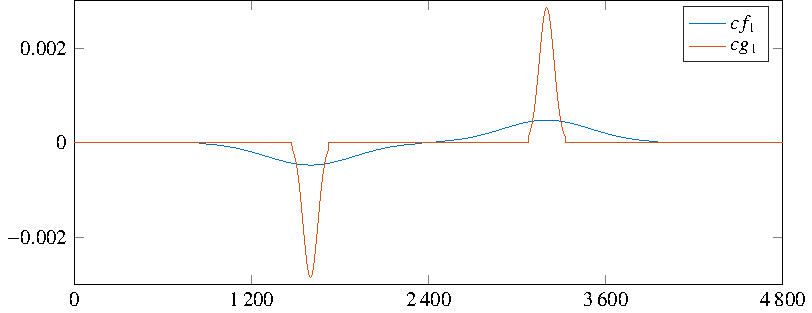
\includegraphics[width=0.9\textwidth]{./papers/deconvolve/pictures/level/level1.pdf}
\caption{Level 1 unverändert\label{deconvolve:level1}}
\end{figure}

Nun wird mit einer geeigneten Manipulation des Vektors $cf_k$ versucht, die blauen Koeffizienten so anzupassen, bis sie den orangen möglichst ähnlich sind.

Man erkennt klar, dass die $cf_1$, also die Koeffizienten des ersten Levels der Funktion $f(x)$ unter einer gewissen Schwelle abgeschwächt und darüber überproportional verstärkt werden müssen.
Die Funktion
$$s(cf_{k,n}) = \left( \frac{cf_{k,n}}{m}\right)^\alpha$$
ist dafür ein vielversprechender Ansatz.
Der Parameter $m$ ist hierbei ebendiese Schwelle und mit $\alpha$ kann die Verstärkung bestimmt werden.
Wird $\alpha = 1$ gewählt soll sich der Koeffizient aber nicht verändern, weshalb man nochmals mit $m$ multiplizieren muss.
$$s(cf_{k,n}) = m\cdot \left( \frac{cf_{k,n}}{m}\right)^\alpha.$$
Ein Problem stellen hier aber noch negative Koeffizienten dar. In diesem Fall kann nur mit ganzzahligen Potenzen gearbeitet werden, da man sonst komplexe Lösungen erhält, welche für diese Anwendung nicht brauchbar sind.
Um dies zu umgehen, muss nur der Betrag von $cf_{k,n}$ gebildet, und dessen Vorzeichen aber noch mit der Signumfunktion mitgenommen werden.
Somit erhalten wir eine Funktion

\begin{align}
s(cf_{k,n})=m\cdot \left(\frac{|cf_{k,n}|}{m}\right)^{\alpha}\cdot \text{sign}(cf_{k,n}), \qquad m,\alpha\in\mathbb{R}
\label{deconvolve:funktion}
\end{align}
als Beziehung zwischen den \glqq unscharfen\grqq{} und \glqq scharfen\grqq{} Koeffizienten.

Abbildung \ref{deconvolve:function} zeigt unsere Funktion aus \eqref{deconvolve:funktion} mit $m=0.75$, verschiedenen $\alpha$ und der Variable $cf_k\in[-1.5;1.5]$.
Gut erkennbar ist darin, wie mit dem Parameter $\alpha$ die Verstärkung justiert werden kann.
Bei $\alpha = 1$ werden die Koeffizienten einfach übernommen.
Auch die Wirkung von $m$ wird klar.
Bei $m=-0.75$ und $m=0.75$ werden die Kurven fixiert.
\begin{figure}
\centering
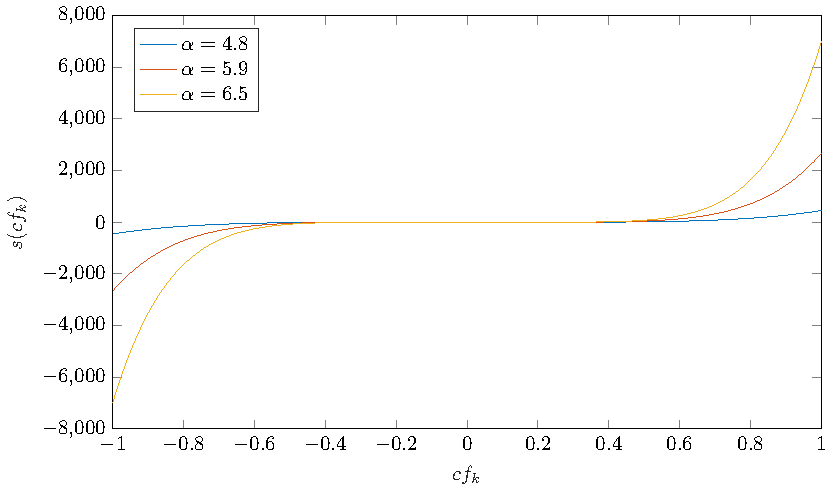
\includegraphics[width=0.9\textwidth]{./papers/deconvolve/pictures/function.pdf}
\caption{Funktion $s(cf_{k,n})$\label{deconvolve:function}}
\end{figure}

Nun soll diese Funktion auf wenn möglich alle verschiedenen Levels unserer Wavelet-Koeffizien\-ten angewendet werden.
Für $m$ kann genau der Schnittpunkt zwischen den beiden Kurven in Abbildung \ref{deconvolve:level1} gewählt werden.
$\alpha$ wird dann so bestimmt, dass die Spitze der blauen Kurve nach der Manipulation mit derjenigen der orangen zusammenfällt.
\begin{figure}
\centering
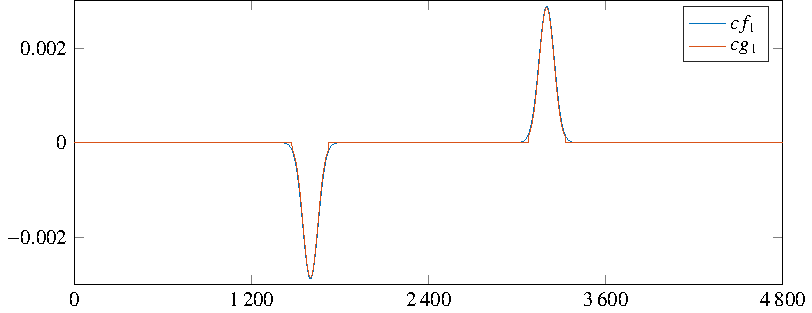
\includegraphics[width=0.9\textwidth]{./papers/deconvolve/pictures/level/level1_n.pdf}
\caption{Level 1 mit veränderten $cf_1$\label{deconvolve:level1_n}}
\end{figure}

Abbildung \ref{deconvolve:level1_n} zeigt die Funktion \eqref{deconvolve:funktion} auf die Elemente von $cf_1$ angewendet.
Der Unterschied zwischen den beiden Kurven ist nur noch schwach erkennbar, die Manipulation scheint auf diesem Level also erfolgreich verlaufen zu sein.

\subsection{Koeffizienten auf höheren Level}

Mit entsprechenden $m$ und $\alpha$ soll nun gleich auf den anderen Level vorgegangen werden.
Abbildung \ref{deconvolve:level5} zeigt Level 5 vor und nach der Koeffizientenmanipulation.
\begin{figure}
\centering
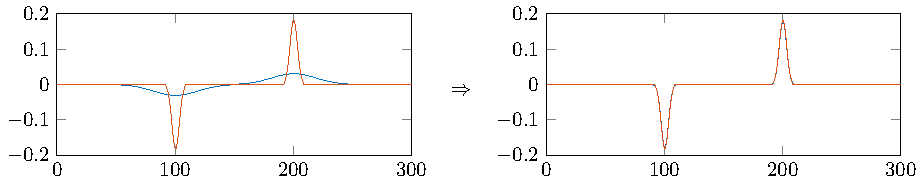
\includegraphics[width=0.9\textwidth]{./papers/deconvolve/pictures/level/level5.pdf}
\caption{Level 5 vorher und nachher\label{deconvolve:level5}}
\end{figure}

Auf diesem Level scheint alles noch wie erwünscht zu funktionieren.
Jeden Schritt höher kommen aber, wie weiter oben angedeutet, weniger (halb so viele) Koeffizienten dazu.
Waren es im ersten noch 4800, so sind es im fünften nur noch 300.
Auf dem Level 13 sind es dann nur noch zwei.
Deswegen wird es immer schwerer, die beiden Freiheitsgrade $m$ und $\alpha$ so zu wählen, dass noch eine Annäherung von $cf_k$ an $cg_k$ resultiert.
Mit dieser Beispielfunktion $f(x)$ war es möglich, mit der Funktion aus \eqref{deconvolve:funktion} bis auf das Level 12 eine Verbesserung zu erreichen.

\subsection{Ergebnis}
Abbildung \ref{deconvolve:result_1d} zeigt unsere ursprüngliche Funktion $f_1(x)$.
Deren Wavelet-Koeffizienten $cf_k$ wurden dann mit der oben beschriebenen Methode bearbeitet, was nach der Rücktransformation zu $f_2(x)$ führt.
Verglichen mit $f_1(x)$, ist $f_2(x)$ deutlich näher an $g(x)$ gerückt.
\begin{figure}
\centering
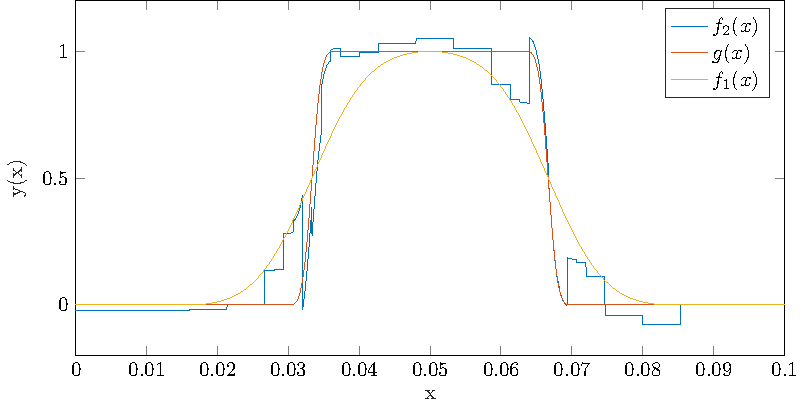
\includegraphics[width=0.9\textwidth]{./papers/deconvolve/pictures/result_1d.pdf}
\caption{Rücktransformation nach durchgeführter Manipulation\label{deconvolve:result_1d}}
\end{figure}

In der Nähe des Randes hat sich die Steilheit tatsächlich vergrössert, allerdings sind weiter weg von diesem Rand zusätzliche Artefakte hinzugekommen.
Um dies besser zu verstehen wird an dieser Stelle die stetige Wavelet-Transformation zur Hilfe genommen.

In Abbildung \ref{deconvolve:cwt} sind diese ersichtlich.
Ein Vergleich der CWT von $g(x)$ und $f_1(x)$ zeigt, dass bei $f_1(x)$ \glqq Masse\grqq{} in die beiden Spitzen, also nach unten, verschoben werden muss.
Das macht mit Einbezug der Fouriertheorie intuitiv Sinn, da ja ein Hinzufügen von hohen Frequenzen die Flankensteilheit erhöht.
Dies ist mit der angewandten Methode natürlich nur beschränkt möglich, da ja jedes Level einzeln behandelt wird.
Die so erzeugten Artefakte sind bei der stetigen Transformation von $f_2(x)$ als vertikale Striche vor allem in der unteren Hälfte erkennbar.
Betrachtet man nur dieses Bild könnte man meinen, dass das Vorgehen erfolgreich war.

\begin{figure}
\centering
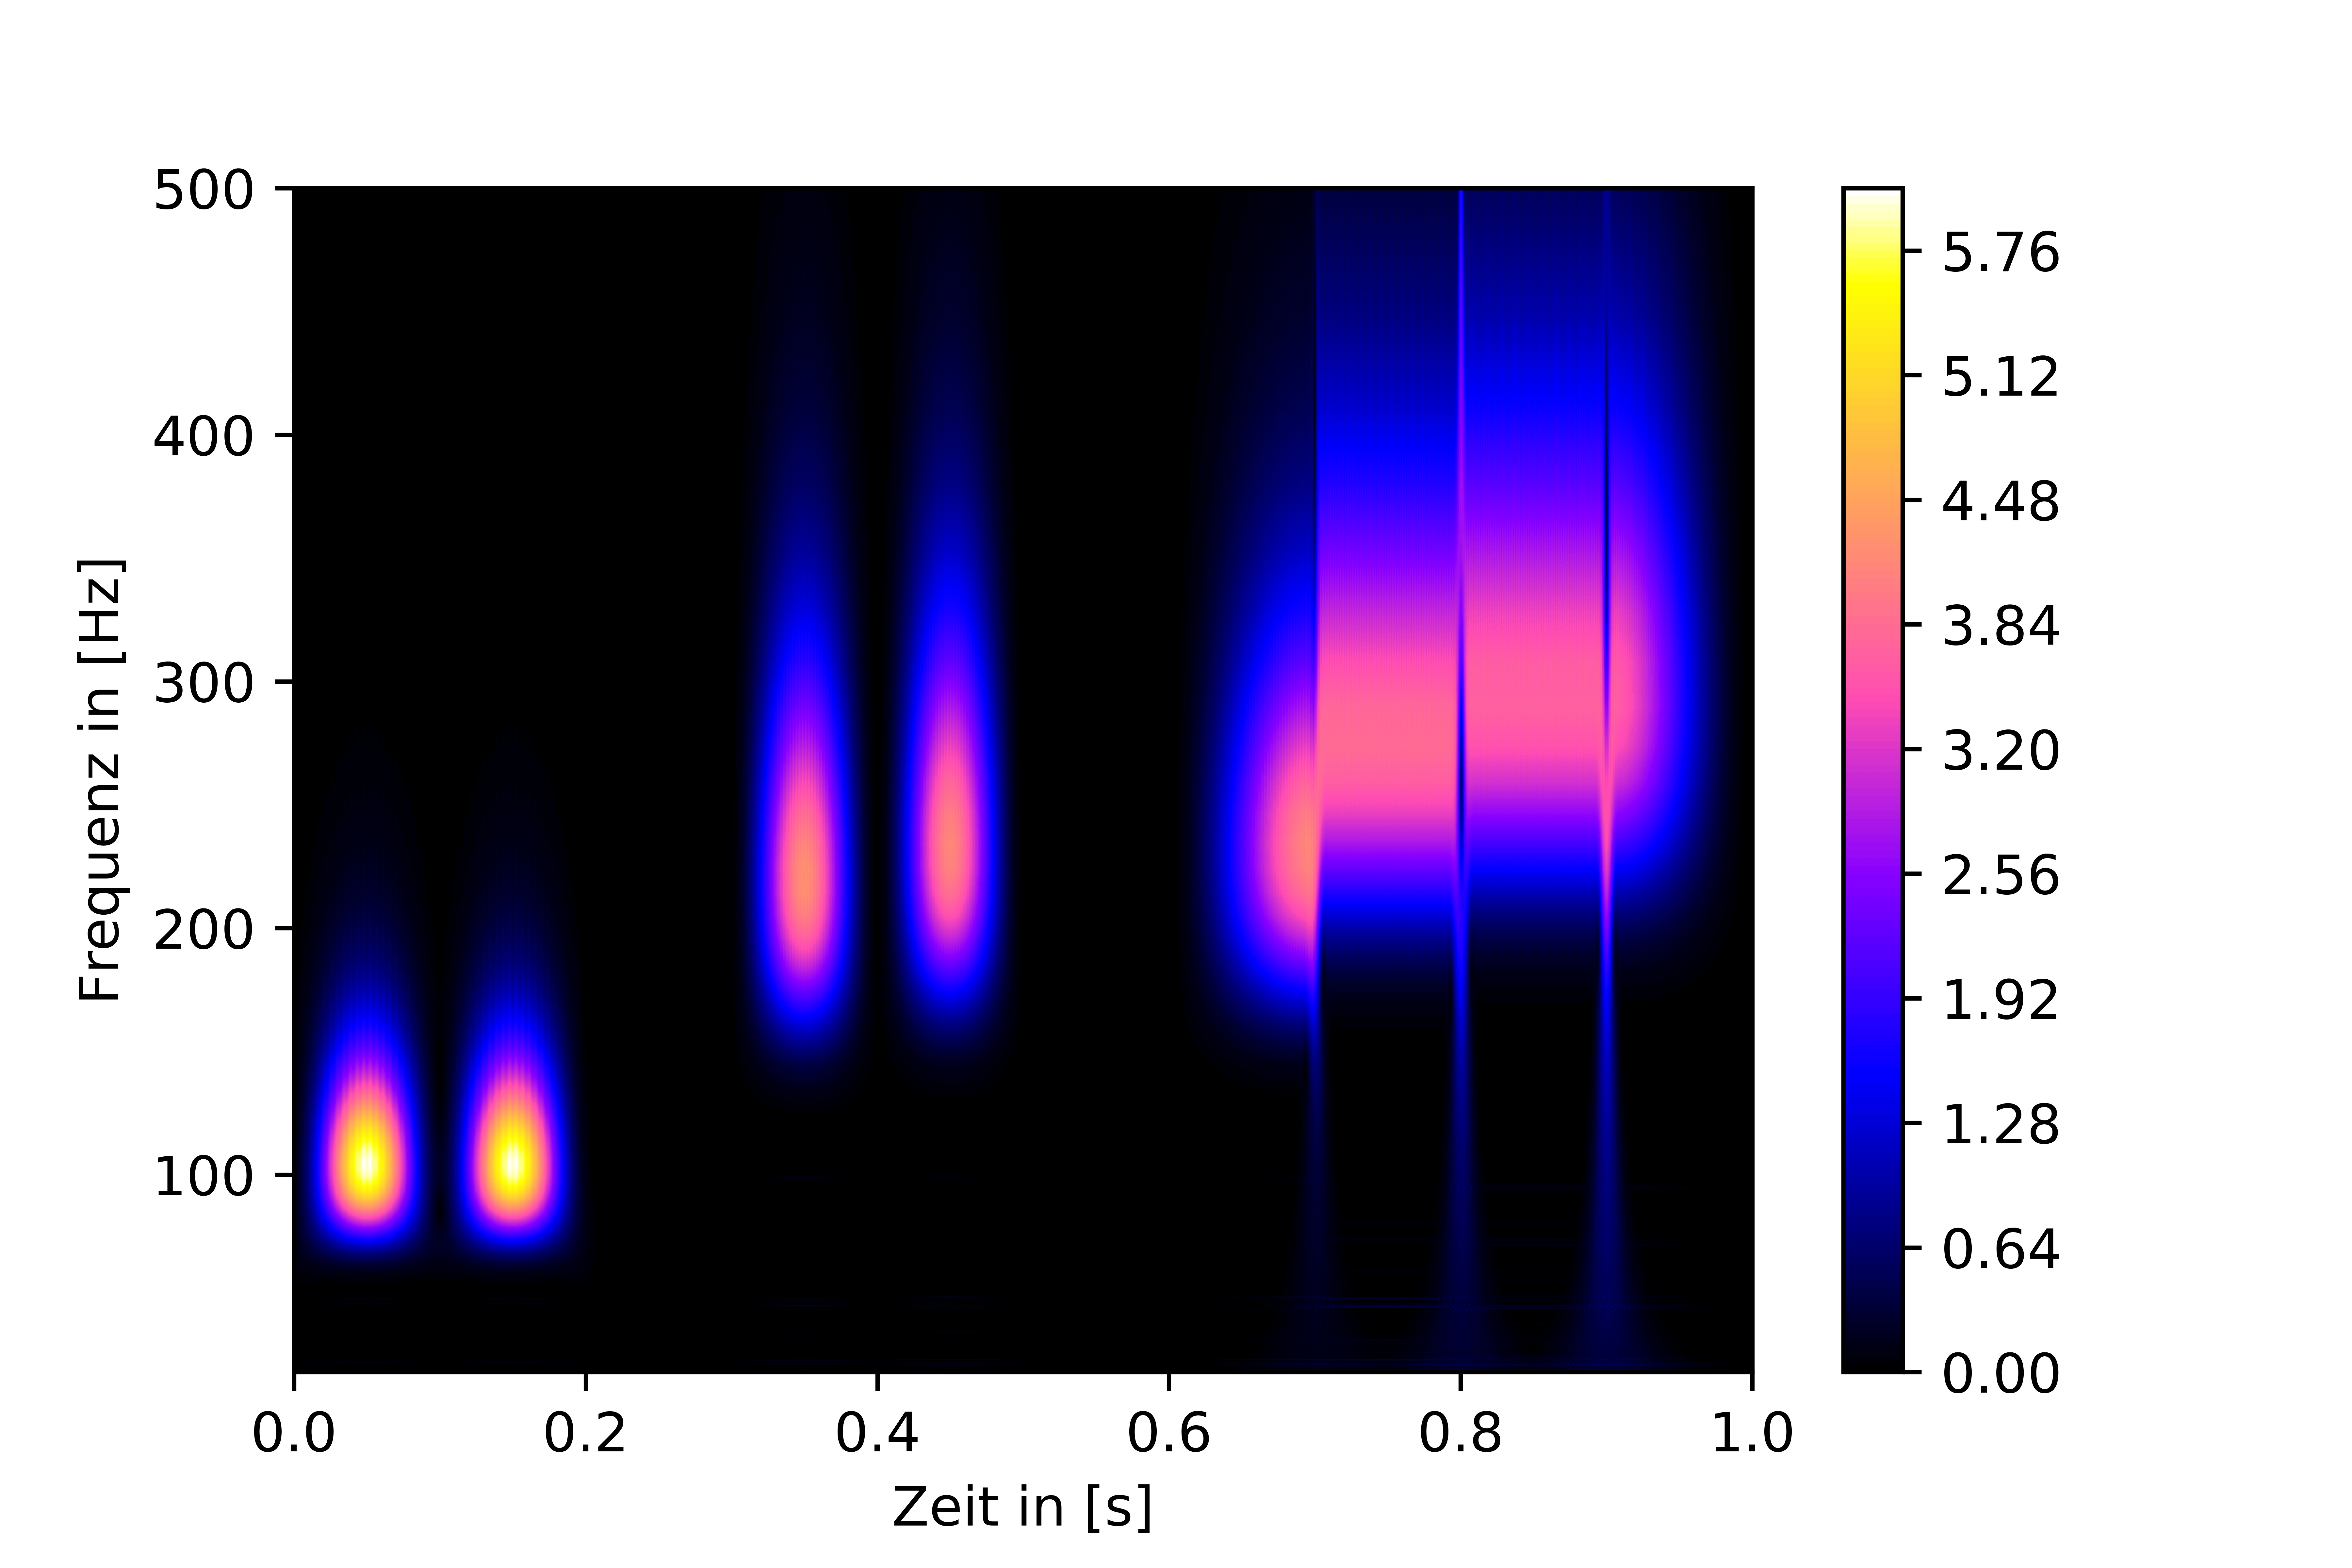
\includegraphics[width=0.9\textwidth]{./papers/deconvolve/pictures/cwt.pdf}
\caption{Stetige Transformationen vor und nach Manipulation\label{deconvolve:cwt}}
\end{figure}

Wie gut man aber wirklich wieder zum Original zurückgekommen ist, sieht man noch deutlicher in der Abbildung mit der Differenz.
Hier sind die Abweichungen zur  scharfen Funktion $g(x)$ nun klar zu erkennen.
Die angewandte Methode hat praktisch über alle Dilatationen eine unerwünschte Änderung zur Folge.
Es ist gut zu erkennen, dass nicht nur direkt am Ort der Änderung, sondern auch \glqq weit \grqq{} weg davon solche unerwünschten Linien entstanden sind.

Das Problem scheint, dass beim Erarbeiten der Methode die Wavelet-Theorie ähnlich wie die Fourier-Theorie behandelt wurde.
Macht man eine Fourier-Transformation, so wirkt sich eine Manipulation im Frequenzbereich automatisch auf den richtigen Ort im Zeitbereich aus.
Bei der Wavelet-Transformation ist dies, wie der Versuch zeigt, nicht der Fall.
Die Ortsinformation geht nicht ganz verloren, wodurch Ort und Frequenz nicht vollständig voneinander getrennt sind.


\section{Anwendung auf ein Bild}
\rhead{Anwendung auf ein Bild}
Auch wenn keine Verbesserung zu erwarten ist, soll dieser Teilerfolg nun ein Bild übertragen werden.
Dabei wird immerhin ersichtlich, wie das Vorgehen auf zwei Dimensionen erweitert werden kann.

Ein schwarz-weiss Bild kann man als Matrix betrachten, dessen Einträge zwischen 0 und 1 für die Helligkeit eines Pixels stehen.
0 entspricht schwarz, 1 entspricht weiss.

Als Versuchsbild wird ein etwas verschwommenes Dreieck, wie abgebildet links in \ref{deconvolve:example} (ohne blauen und orange Linie) verwendet.
Die Grösse beträgt $9600\times9600$ Pixel, analog den 9600 Samples der Funktion $f(x)$ aus Abbildung \ref{deconvolve:1d}.
\begin{figure}[h]
\centering
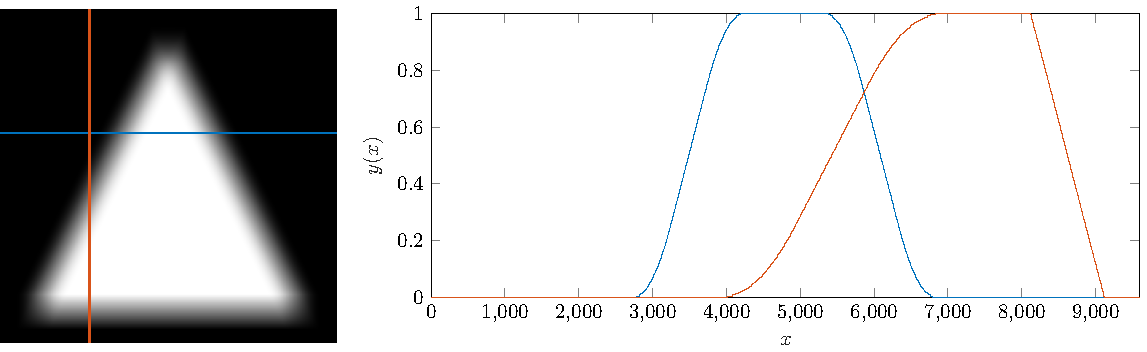
\includegraphics[width=0.9\textwidth]{./papers/deconvolve/pictures/dreieck.pdf}
\caption{Beispielbild und eindimensionale Interpretation\label{deconvolve:example}}
\end{figure}

Man folge in Abbildung \ref{deconvolve:example} beim Dreieck der blau markierten \glqq Zeile\grqq{}.
Reiht man diese Werte von links nach rechts auf, kommt man auf die blaue Kurve rechts in der Abbildung.
Analog kommt man auf die orange Kurve, wenn man der orangen \glqq Spalte\grqq{} folgt.
Vorteil diese Bildes ist also offensichtlich, dass man dessen zugehörige Matrix Zeilen- und Spaltenweise gleich wie das eindimensionale Signal betrachten kann.

Die Parameter $m$ und $\alpha$, die vorher für jedes Level einzeln bestimmt wurden, bleiben erhalten.
Die Funktion $s(cf_{k,n})$ aus \eqref{deconvolve:funktion} wird also auf alle Level gleich wie beim eindimensionalen Signal angewendet.
Dies geschieht einmal Zeilen- und Spaltenweise, es wird also insgesamt 19200 mal eine Analyse mit der diskreten Wavelet-Transformation durchgeführt.
Sind $f_\text{rows}(x,y)$ und $f_\text{cols}(x,y)$ die Zeilen-, bzw. Spaltenweise \glqq geschärften\grqq{} Varianten des ursprünglichen Bildes, kann davon das arithmetische Mittel genommen werden
$$f_\text{sharp}(x,y)=\frac{f_\text{rows}(x,y)+f_\text{cols}(x,y)}{2},$$
wobei $f_\text{sharp}(x,y)$ das so erhaltene Endresultat bezeichnet.

Nun ist zu erwarten dass die im vorherigen Abschnitt aufgetretenen Artefakte auch hier wieder in Erscheinung treten.
Abbildung \ref{deconvolve:ergebnis} zeigt das Ergebnis.
\begin{figure}[h]
\centering
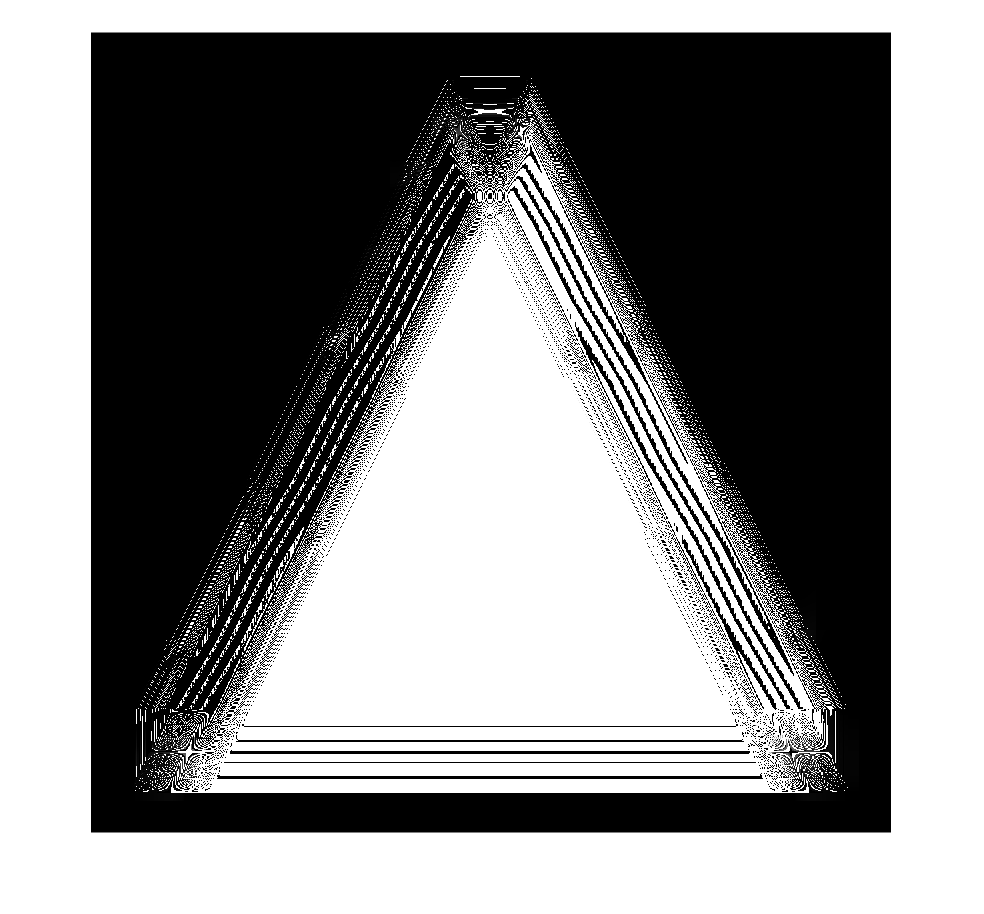
\includegraphics[width=0.7\textwidth]{./papers/deconvolve/pictures/dreieck_sharp.png}
\caption{Mit $s(cf_{k,n})$ \glqq geschärftes\grqq{} Bild\label{deconvolve:ergebnis}}
\end{figure}
 
Eine Verbesserung ist wie vorherzusehen nicht zu erkennen. Wo vorher der Rand verschwommen war, sind jetzt einfach starke Schwingungen aufgetaucht.

\section{Schlussfolgerung}
\rhead{Schlussfolgerung}
Innerhalb dieser Seminararbeit konnte keine fertige Funktion zur Bildschärfung erarbeitet werden.
Der bestehende Ansatz mit der Beziehung \eqref{deconvolve:funktion}, welche zwei Freiheitsgrade beinhaltet, könnte aber noch verfeinert werden.
Die beiden Parameter $m$ und $\alpha$ wurden hier mithilfe einer eindimensionalen Funktion $g(x)$ (Abbildung \ref{deconvolve:1d}) festgelegt.
Es wäre daher vielleicht möglich, durch geschickteres wählen dieser Parameter auf ein besseres Ergebnis zu kommen.
Ausserdem ist die Anwendung auf das Bild noch nicht ausgereift.

Es wurden auch nur das Haar- bzw. db1-Wavelet verwendet.
Ein ähnlicher Ansatz, z.B. mit höheren Debauchies-Wavelets wäre sicher ein Versuch Wert.

Die Hauptursache für das unbefriedigende Resultat liegt im allgemeinen aber woanders.
Es wurde nur versucht, die Koeffizienten auf den einzelnen Level zu verändern, bzw jede Zeile in Abbildung \ref{deconvolve:y1_cwt} wurde unabhängig von der benachbarten verstärkt oder geschwächt.

Eine bessere Methode würde berücksichtigen, dass die Wavelet-Transformation ja zwei Dimensionen hat (Dilatation $a$ und Translation $b$) und somit \glqq Masse \grqq{} in der Ebene, also zwischen Level und nicht nur auf einer Zeile nach links oder rechts verschoben werden muss.
Ändert man auf einem Level etwas, so muss die Auswirkung auf die anderen Level unbedingt berücksichtigt werden.


Es ist somit problematisch, die Wavelet-Transformation ähnlich wie die Fourier-Transformation zu behandeln.
Ein verändern eines Koeffizienten an einer bestimmten Stelle bewirkt nicht nur dort, sondern auch bei anderen Frequenzen oder genauer Dilatationen etwas.
Genau dies konnte ja beim Versuch mit der eindimensionalen Funktion beobachtet werden.



%\printbibliography[heading=subbibliography]
\end{refsection}
